\chapter{触觉} \label{chap:chap19}

在关于触觉的这一章中,我们将重点放在手上,因为它对感知这种方式很重要,特别是在物体特性的感知和熟练动作表现中的作用。
人手是进化的伟大创造之一。
我们手指的精细操作能力之所以成为可能,是因为它们具有精细的感觉能力;
如果我们失去了手指的触觉,就失去了手的灵活性。



\textit{光滑皮肤}的柔软度和顺应性在触觉中起着重要作用。
当物体接触手时,皮肤会按照其轮廓形状变形,形成物体表面的镜像。
由此产生的皮肤位移和凹陷会拉伸组织,从而刺激接触区域或接触区域附近机械受体的感觉末梢。



这些受体高度敏感,并在我们用手操纵物体和探索世界时持续活跃。
它们向大脑提供有关物体在手中的位置、形状和表面纹理、施加在接触点的力大小,以及手或物体移动时这些特征如何随时间变化的信息。
指尖是身体中神经支配最密集的部位之一,为手操作的物体提供了广泛而冗余的体感信息。


此外,手的解剖结构具有多个关节和可合并的手指,使人类能够以反映物体整体形状的方式塑造手,从而提供以手为中心的外部世界的本体感觉表征。
这种内化物体形状的能力使我们能够创造出可以单独扩展我们双手能力的工具。


当我们熟练使用手术刀或剪刀等工具时,会感觉到工具工作表面的状况,就好像我们的手指在那里一样,因为 2 组触觉受体检测到了这些远处条件产生的振动和力。
当我们用手指在一个表面上滑动时,我们会感觉到它的形状和质地,因为另一组机械受体具有高空间和时间分辨率。
盲人利用这种能力以每分钟一百字的速度阅读盲文。
当我们握住和操纵一个物体时,我们会非常小心地使用所需的力,因为特定的机械受体会持续监控滑动并适当调整我们的抓握。


我们还能够仅通过触摸来识别放在手中的物体。
当我们拿到棒球时,由于它的形状、大小、重量、密度和质地,我们无需看就能立即认出它。
我们不必考虑每个手指提供的信息就可以推断出该物体一定是棒球;
信息流入记忆并立即匹配先前存储的棒球表示。
即使我们以前从未接触过棒球,我们也会将其感知为一个单一物体,而不是一组离散的特征。
大脑的体感通路有一项艰巨的任务,即整合每只手上成千上万个传感器的信息,并将其转化为适合认知和行动的形式。


感觉信息被提取出来,既用于运动控制,也用于认知,并且针对这些目的提取出了不同类型的信息。
例如,我们可以将注意力从棒球的形状转移到它在手中的位置,以重新调整我们的握持,以进行有效的投掷或投球。
这种对感觉信息不同方面的选择性关注是由皮层机制引起的。



\section{主动触觉和被动触觉有不同的目标}

触觉被定义为 2 个物体之间的直接接触。
在神经科学中,触觉是指有意识地感知与身体接触的特殊感觉。
触觉可以是主动的,例如当您将手或身体的其他部分移动到另一个表面时;
也可以是被动的,例如当某人或其他东西触摸您时。
% 受试者是意识的一个代理?
\textit{主动触觉}从根本上说是一个\textit{自上而下}的过程,在这个过程中,受试者具有主动性,寻求特定信息,并控制发生的事情。
受试者选择目标的相关显著特征来确定后续行为。
他们选择要抓取的物体和获得它所需的最有效的手型,并决定如何操纵它以实现特定目标。
在主动触觉中,体感信息描述了物体的物理特性以及受试者手和手臂的运动行为,以及它们与任务目标的关系。
重要的是,物体的主动操作是基于触摸作为一种三维模态的概念,旨在捕捉物体的体积、地形和弹性特性,正如\textit{罗伯塔$\cdot$克莱兹基}和\textit{苏珊$\cdot$莱德曼}首次提出的那样。
这些三维特性最好通过主动操作来领会,包括用手抓握、旋转和轮廓追踪。


被动触觉采用自下而上的过程,在该过程中,受试者对实验者或临床医生指定的外部刺激做出响应。
实验者选择并控制传递到皮肤的刺激的位置、幅度、力量、时机、持续时间和空间范围。
随后的行为由范例中提供的指令指导。
触觉刺激分为实验者选择的类别和/或按照强度或愉悦程度的标度进行评级。
因此,受试者需要分析所有传递的体感信息,并在部分任务说明的指导下选择特定特征。


触觉刺激的主动和被动模式会激活皮肤中相同的受体群,并在感觉神经纤维中引起类似的响应。
它们在反映刺激期间注意力和行为目标的认知特征上有所不同。
通过说出物体的名称或描述感觉来测试被动触觉;
当手操纵物体时使用主动触觉。
触觉的感觉和运动组成部分在大脑解剖学上密切相关,并且在指导运动行为方面具有重要的功能。


在主动触觉中,来自大脑皮层运动中枢的下行纤维终止于位于中央背角的内部神经元,这些内部神经元从皮肤接收触觉信息。
来自皮层运动区的纤维终止于\textit{脊髓背根核},提供产生行为的运动指令的外发副本(或\textit{伴随发送})(第~\ref{chap:chap30}~章)。
通过这种方式,由于受试者手部运动而产生的手部触觉信号可以在神经学检查或心理物理测试中在中枢区别于被动施加的刺激。


当患者手部出现缺陷时,区分主动和被动触觉之间的区别在临床上很重要。
感觉丧失可能导致无力、僵硬或笨拙等运动功能障碍,因此被动感觉测试在神经系统检查中很重要。
常见的触觉神经学测试包括检测阈值、振动感、两点或纹理辨别,以及通过触摸识别形状(立体感)的能力。 
这些测试衡量了各种触觉受体的灵敏度和功能。
与预期值的偏差可能有助于诊断底层感觉缺陷或导致体感功能障碍的病变。
本章讨论了这些测试背后的神经机制。
其他常见的体感功能测试(肌腱反射、针刺和热测试)在其他章节中讨论。



\section{手有 4 种类型的机械受体}

如图~\ref{fig:19_1}~所示,人手的触觉感觉来自 4 种机械受体:\textit{梅斯诺小体}、\textit{梅克尔细胞}、\textit{环层小体}和\textit{鲁菲尼终末器}。
每个受体根据其形态、神经支配模式和皮肤深度以独特的方式做出响应。
触觉可以理解为这 4 个系统协同作用所提供信息的综合结果。


\begin{figure}[htbp]
	\centering
	\includegraphics[width=0.95\linewidth]{chap19/fig_19_1}
	\caption{4 种类型的机械受体负责人手的触觉。
		支配手部的有髓感觉神经末端被专门的结构包围,这些结构可以检测皮肤上的触感。
		这些受体在形态、神经支配模式、皮肤位置、感受野大小和对触觉的生理响应方面各不相同\cite{johansson1983tactile}。
		A. 手部光滑(无毛)皮肤的表层和深层各包含不同类型的机械受体。
		表层包含小受体细胞:梅斯诺小体(\textit{快适应1型})和梅克尔细胞(\textit{慢适应1型})。
		支配这些受体的感觉神经纤维具有支配一种类型的多个受体的分支末端。
		皮肤和皮下组织的深层包含大受体:\textit{环层小体}(\textit{快适应2型})和\textit{鲁菲尼终末器}(\textit{慢适应2型})。
		这些受体中的每一个都由一根神经纤维支配,而每根纤维仅支配一个受体。
		B. 机械受体的感受野反映了其末端在皮肤中的位置和分布。
		皮肤表层的触觉受体比深层的受体具有更小的感受野。
		C. 支配每种机械受体的神经纤维在被激活时的响应不同。
		脉冲序列示意图显示了通过对皮肤缓慢增加恒定的压力激活其受体时,每种类型神经的响应。
		\textit{快适应}纤维在压力刺激开始和结束时对运动做出响应,并迅速适应持续的刺激,而\textit{慢适应}纤维对稳定压力和运动都有响应,并缓慢适应。}
	\label{fig:19_1}
\end{figure}


触觉受体由\textit{慢适应}或\textit{快适应}的轴突支配。
如图~\ref{fig:19_1}~和表~\ref{tab:19_1}~所示,\textit{慢适应}纤维通过持续放电响应稳定的皮肤压迫,而\textit{快适应}纤维在压迫停止时停止放电。
因此,手部持续的机械感觉主要来自\textit{慢适应}纤维;
皮肤上或横跨皮肤的运动感觉主要由\textit{快适应}纤维传递。


\begin{table}[htbp]
	\caption{光滑皮肤中的皮肤机械受体} \label{tab:19_1} \centering
	\begin{tabular}{lllll}
		\toprule
		 & 类型 1 &  & 类型 2 & \\
		 \toprule
		 & 慢适应类型 1 & 快适应类型 1  & 慢适应类型 2 & 快适应类型 2 \\
		\midrule
		受体 & \makecell[l]{梅克尔细胞/\\轴突复合体\\(多末端)} & \makecell[l]{梅斯诺小体\\(多末端)} & \makecell[l]{鲁菲尼终末器\\(单末端)} & \makecell[l]{环层小体\\(单末端)} \\
		位置 & \makecell[l]{围绕汗腺的\\中间脊底部} & \makecell[l]{真皮乳头(\\邻近限制脊)} & \makecell[l]{皮肤褶皱、关节\\处皮肤、指甲床} & \makecell[l]{真皮(\\深层组织)} \\
		\makecell[l]{轴突直径\\(微米)} & 7-11 & 6-12 & 6–12 & 6–12 \\
		\makecell[l]{传导速度\\(毫秒)} & 40–65 & 35–70 & 35–70 & 35–70 \\
		最佳刺激 & 边、点 & 横向运动 & 皮肤拉伸 & 震动 \\
		\makecell[l]{对持续压\\痕的响应} & \makecell[l]{持续且适应\\缓慢(不规则\\激活模式)} & \makecell[l]{刺激开始\\时的阶段性} & \makecell{持续且适应\\缓慢(正常\\激活速率)} & \makecell[l]{刺激开始\\时的阶段性} \\
		\bottomrule
	\end{tabular}
\end{table}


手上的触觉受体根据在皮肤中的大小和位置进一步细分为 2 种类型。
如图~\ref{fig:19_2},表~\ref{box:19_1}~所示,类型1的触觉纤维终止于皮肤表层的真皮和表皮之间边缘的小受体器官簇(梅斯诺小体或梅克尔细胞)。
\textit{快适应1型} 纤维是最常见的触觉传入纤维,在人和猴子的指尖密度约为每平方厘米150根;
\textit{慢适应1型}纤维也广泛分布在手部,指尖的密度为每平方厘米 70 根。


\begin{proposition}[指纹结构提高了手部的触觉敏感性] \label{box:19_1}
	
	\quad \quad 光滑皮肤的组织结构(手掌和指尖的光滑无毛皮肤)在手对触觉的敏感性中起着至关重要的作用。
	如图~\ref{fig:19_3}~所示,指纹是由表皮中一组平行脊构成,即乳头脊。
	从每个脊的中心,排列整齐的\textit{梅克尔细胞}位于汗管下方,形成了一个空间网格,使我们能够准确地在指尖上定位刺激。
	
	\quad \quad 每个脊都被表皮褶皱(限制脊)环绕,这些限制脊在手指、手掌和脚底上可见为细线。
	限制脊增加了皮肤的硬度和刚度,保护皮肤在接触物体或赤脚行走时免受损伤。
	梅斯诺小体通常位于毗邻限制脊的真皮乳头中;
	如图~\ref{fig:19_4}~所示,每个真皮乳头包含多个梅斯诺小体,并由两到 5 个\textit{快适应1型}轴突提供神经支配。
	
	\quad \quad \textit{梅克尔细胞}由\textit{慢适应 1 型}纤维支配,密集地聚集在每个乳头脊的中心,位于表皮汗腺管周围的中间脊底部(图~\ref{fig:19_4}A),使它们处于一个极佳的位置,可以检测表皮因压力或侧向拉伸而导致的变形。
	它们的触觉感受功能类似于毛发皮肤触觉小结中的\textit{梅克尔细胞}(第~\ref{chap:chap18}~章)。
	
	\quad \quad 指纹给光滑皮肤增加了波纹、粗糙的结构,增加了摩擦力,使我们能够在抓取物体时避免滑动。
	当这些脊与物体的纹理表面接触时,摩擦力进一步增加。
	光滑的表面很容易在手指下方滑动,因此需要更大的握力来保持手部的稳定性;瓶盖上的螺纹通常是脊状结构,以便于转动。
	当我们触摸物体时,限制脊和物体之间的摩擦力也会增强我们对表面特征的感知,产生的振动使我们能够检测到微小的不规则性,如木纹和织物纤维。
	
	\quad \quad 乳头脊的规则间距(以及特定受体在该网格内的精确定位)使我们能够通过手的来回运动反复扫描表面,同时保持相邻表面特征的恒定空间对齐。
	它们还为参照触觉刺激的精确位置提供了解剖网格。
	
\end{proposition}


\begin{figure}[htbp]
	\centering
	\includegraphics[width=1.0\linewidth]{chap19/fig_19_4}
	\caption{光滑和毛发皮肤中梅斯诺小体和梅克尔细胞的神经支配模式。
		A. 人类指尖皮肤中一个乳头脊的共聚焦横截面显示了机械受体的神经支配模式。
		梅斯诺小体位于限制脊边缘下方的真皮乳头中(蓝色),由 2 种或多种\textit{快适应1型}纤维支配。
		当纤维进入受体囊时,它们失去了髓鞘(橙色),暴露出广泛的末端球茎(绿色),感受转换发生在这些末端球茎上。
		单个\textit{慢适应 1 型}纤维支配聚集在中间脊底部的\textit{梅克尔细胞}群,为施加于该脊的压力提供信号。比例尺=50微米。}
		B. 更高倍率的显微照片描绘了角蛋白-8抗体标记的\textit{梅克尔细胞}(红色),其由标记有神经丝重多肽(NFH+)的\textit{慢适应 1 型}纤维(绿色)支配。
		每个神经纤维平行于皮肤表面延伸多个分支,使其能够整合来自皮肤小区域中多个受体细胞的触觉信息。
		每个\textit{梅克尔细胞}的直径约为10微米。
	\label{fig:19_4}
\end{figure}


类型2的纤维稀疏地支配皮肤,并终止于位于真皮或皮下组织中的单个大型受体(\textit{环层小体}和\textit{鲁菲尼终末器})。 
这些受体比类型 1 纤维的受体器官更大但数量更少。
类型2受体尺寸较大,使它们能够在距感觉神经末梢一定距离处感知皮肤的机械位移。
人手指中\textit{快适应2型}纤维的密度仅为每平方厘米21根;
\textit{慢适应2型}纤维含量最少,每平方厘米仅提供 9 根纤维。


\begin{figure}[htbp]
	\centering
	\includegraphics[width=0.85\linewidth]{chap19/fig_19_2}
	\caption{人类光滑皮肤的触觉神经支配。
		光滑皮肤的横截面显示了人手触摸的主要受体。
		所有这些受体均受大直径A$\beta$髓鞘纤维的支配。
		\textit{梅斯诺小体}和\textit{梅克尔细胞}位于表皮底部的皮肤表层,距离皮肤表面0.5至1.0毫米。
		梅斯纳小体位于毛乳头中,与每个乳头脊的边缘接壤。默克尔细胞沿着乳头脊的中心在汗腺导管周围的中间脊下方形成致密带。
		支配这些受体的\textit{快适应1型}和\textit{慢适应1型}纤维在其末端分支,因此每根纤维都支配附近的几个受体器官。
		\textit{环层小体}和\textit{鲁菲尼终末器}位于真皮内(2-3毫米厚)和更深的组织中。
		支配这些受体的\textit{快适应2型}和\textit{慢适应2型}纤维各自仅支配一个受体器官。}
	\label{fig:19_2}
\end{figure}


\begin{figure}[htbp]
	\centering
	\includegraphics[width=0.7\linewidth]{chap19/fig_19_3}
	\caption{人类指尖的皮肤。
		A. 人类食指指纹的扫描电子显微照片。
		手部的光滑皮肤由\textit{乳头脊}和间隔有规律的沟(\textit{限制脊})排列而成。
		汗珠从\textit{乳头脊}中心的导管中渗出,沿着每个隆起的中心形成规则间隔的网格状图案。
		如图~\ref{fig:19_2}~所示,\textit{梅克尔细胞}位于表皮底部汗管下方的密集簇中,沿着\textit{乳头脊}的中心。
		 B. 平行于皮肤表面切割的光滑皮肤的组织切片。
		 此处对胆碱酯酶进行免疫染色的\textit{梅斯诺小体}沿着与\textit{限制脊}相邻的每个\textit{乳头脊}的两侧形成规则间隔的链。
		 因此,\textit{梅斯诺小体}和\textit{梅克尔细胞}形成交替的\textit{快适应 1 型}和\textit{慢适应1型}触摸受体带,跨越每个指纹脊\cite{bolanowski2003organization}。}
	\label{fig:19_3}
\end{figure}



\subsection{细胞的感受野决定了它的触觉敏感区}

单个机械受体纤维从称为感受野的有限皮肤区域传递信息(第~\ref{chap:chap18}~章)。
\textit{亚克$\cdot$威尔波}和\textit{罗兰$\cdot$约翰逊}首先使用微神经图描技术研究了人手的触觉感受野。
他们将微电极通过皮肤插入人类前肢的\textit{正中神经}或\textit{尺神经},并记录单个传入纤维的响应。
他们发现,与其他灵长类动物一样,人类的触觉受体在生理响应和感受野结构方面都存在重要差异。


如图~\ref{fig:19_5}~所示,1 型纤维的感受野小且高度局限,有多个高敏感点,这些点反映了其轴突末稍在皮肤中的分支模式。
一个\textit{快适应1型}轴突通常支配 10 到 20 个\textit{梅斯诺小体},整合来自多个相邻指纹脊的信息。
如图~\ref{fig:19_4}B~所示,一根\textit{慢适应1型}纤维在成年人中支配大约 20 个\textit{梅克尔细胞};
随着年龄的增长,\textit{梅克尔细胞}的数量会显著减少。


\begin{figure}[htbp]
	\centering
	\includegraphics[width=1.0\linewidth]{chap19/fig_19_5}
	\caption{人手的感受野在指尖处最小。
		手上的每个彩色区域表示单个感觉神经纤维的感受野\cite{johansson1983tactile}。
		在皮肤表层,1 型受体的感受野包括斑点状皮肤斑块。
		在深层,2 型感受野延伸到广泛的皮肤区域(浅色阴影),但直接在受体上方的皮肤(黑点)的响应最强。 
		箭头指示激活\textit{慢适应2型}纤维的皮肤拉伸方向。
		C. 整个感受野的压力敏感度显示为等高线图。
		最敏感的区域以深红色表示,最不敏感的区域以淡粉色表示。
		\textit{快适应} 1 型纤维(上图)的感受野有许多高灵敏度点,标记了由纤维支配的迈斯纳小体群的位置。
		\textit{快适应} 2 型纤维(下图)的感受野在\textit{环层小体}上有一个最大灵敏度的单点。
		\textit{慢适应 1 型}纤维的感受野等高线图与\textit{快适应}1 纤维相似。
		同样,\textit{慢适应2型}纤维的感受野图与 \textit{快适应}2 纤维相似。}
	\label{fig:19_5}
\end{figure}


相比之下,支配皮肤深层的 2 型纤维仅与单个\textit{环层小体}或\textit{鲁菲尼终末器}相连。
由于这些受体较大,它们从更广泛的皮肤区域收集信息。 
如图~\ref{fig:19_5}~所示,它们的感受野通常包含一个单一的“热点”,即触觉最敏感的点;
该点位于受体的正上方。


指尖的感受野在人体上是最小的,\textit{慢适应1型}纤维的平均感受野为 11 平方毫米,\textit{快适应1型} 纤维为 25 平方毫米。
小的感受野与指尖上高密度的受体相辅相成。
\textit{近端指骨}和手掌的感受野逐渐变大,这与这些区域的机械受体密度较低的情况相一致。
重要的是,1 型纤维的感受野明显小于大多数接触手的物体,因此仅表示物体有限部分的空间特性。
与视觉系统一样,物体的空间特征分布在一群受刺激的受体上,这些受体的响应在大脑中整合,形成统一的知觉。


每个\textit{快适应2型}轴突在没有分支的情况下终止于单个\textit{环层小体},并且每个 \textit{环层小体}只接受一个\textit{快适应2型} 轴突。
如图~\ref{fig:19_8}A1~所示,\textit{环层小体}是像洋葱一样的大结构,其中连续的结缔组织层被充满液体的空间隔开。
这些层包围着未髓鞘化的\textit{快适应2型} 末端及其有髓鞘的轴突,直至一个或多个朗飞节。
囊膜会放大高频振动,这对使用工具非常重要。
据估计,人手中的 \textit{环层小体}数量从年轻人的 2,400 个到老年人的 300 个不等。


\textit{慢适应2型}纤维支配集中在手指和腕关节、指甲周围皮肤和手掌皮肤褶皱处的\textit{鲁菲尼终末器},。
\textit{鲁菲尼终末器}是长梭形结构,包含从皮下组织延伸到关节、手掌或指甲边缘皮肤褶皱处的胶原纤维。
\textit{慢适应2型}神经末梢像高尔基腱器官(表~\ref{box:32_4})一样交织在囊膜的胶原纤维之间,当沿其长轴拉伸皮肤时会被激发。



\subsection{两点辨别测试测量触觉敏锐度}

人类分辨纹理表面空间细节的能力取决于身体的哪个区域被接触。
当一对探针在手上相距几毫米时,每个探针都被视为一个不同的点,因为它在皮肤上产生一个单独的凹坑,并刺激不重叠的受体群。
当探头靠得更近时,2 种感觉会变得模糊,因为 2 个探头都包含在相同的感受野中。
触觉刺激之间的空间相互作用构成了两点辨别和纹理识别的神经学测试的基础。


在年轻人的指尖上,触觉敏锐度的阈值(即在偶然和完美判别之间定义表现的分隔)约为 1 毫米,但在老年人中下降到约 2 毫米。
指尖和嘴唇的触觉敏锐度最高,感受野最小。
如图~\ref{fig:19_6}A~所示,身体近端部位的触觉敏锐度随着\textit{慢适应1型}和\textit{快适应 1 型}纤维感受野的大小而降低。


\begin{figure}[htbp]
	\centering
	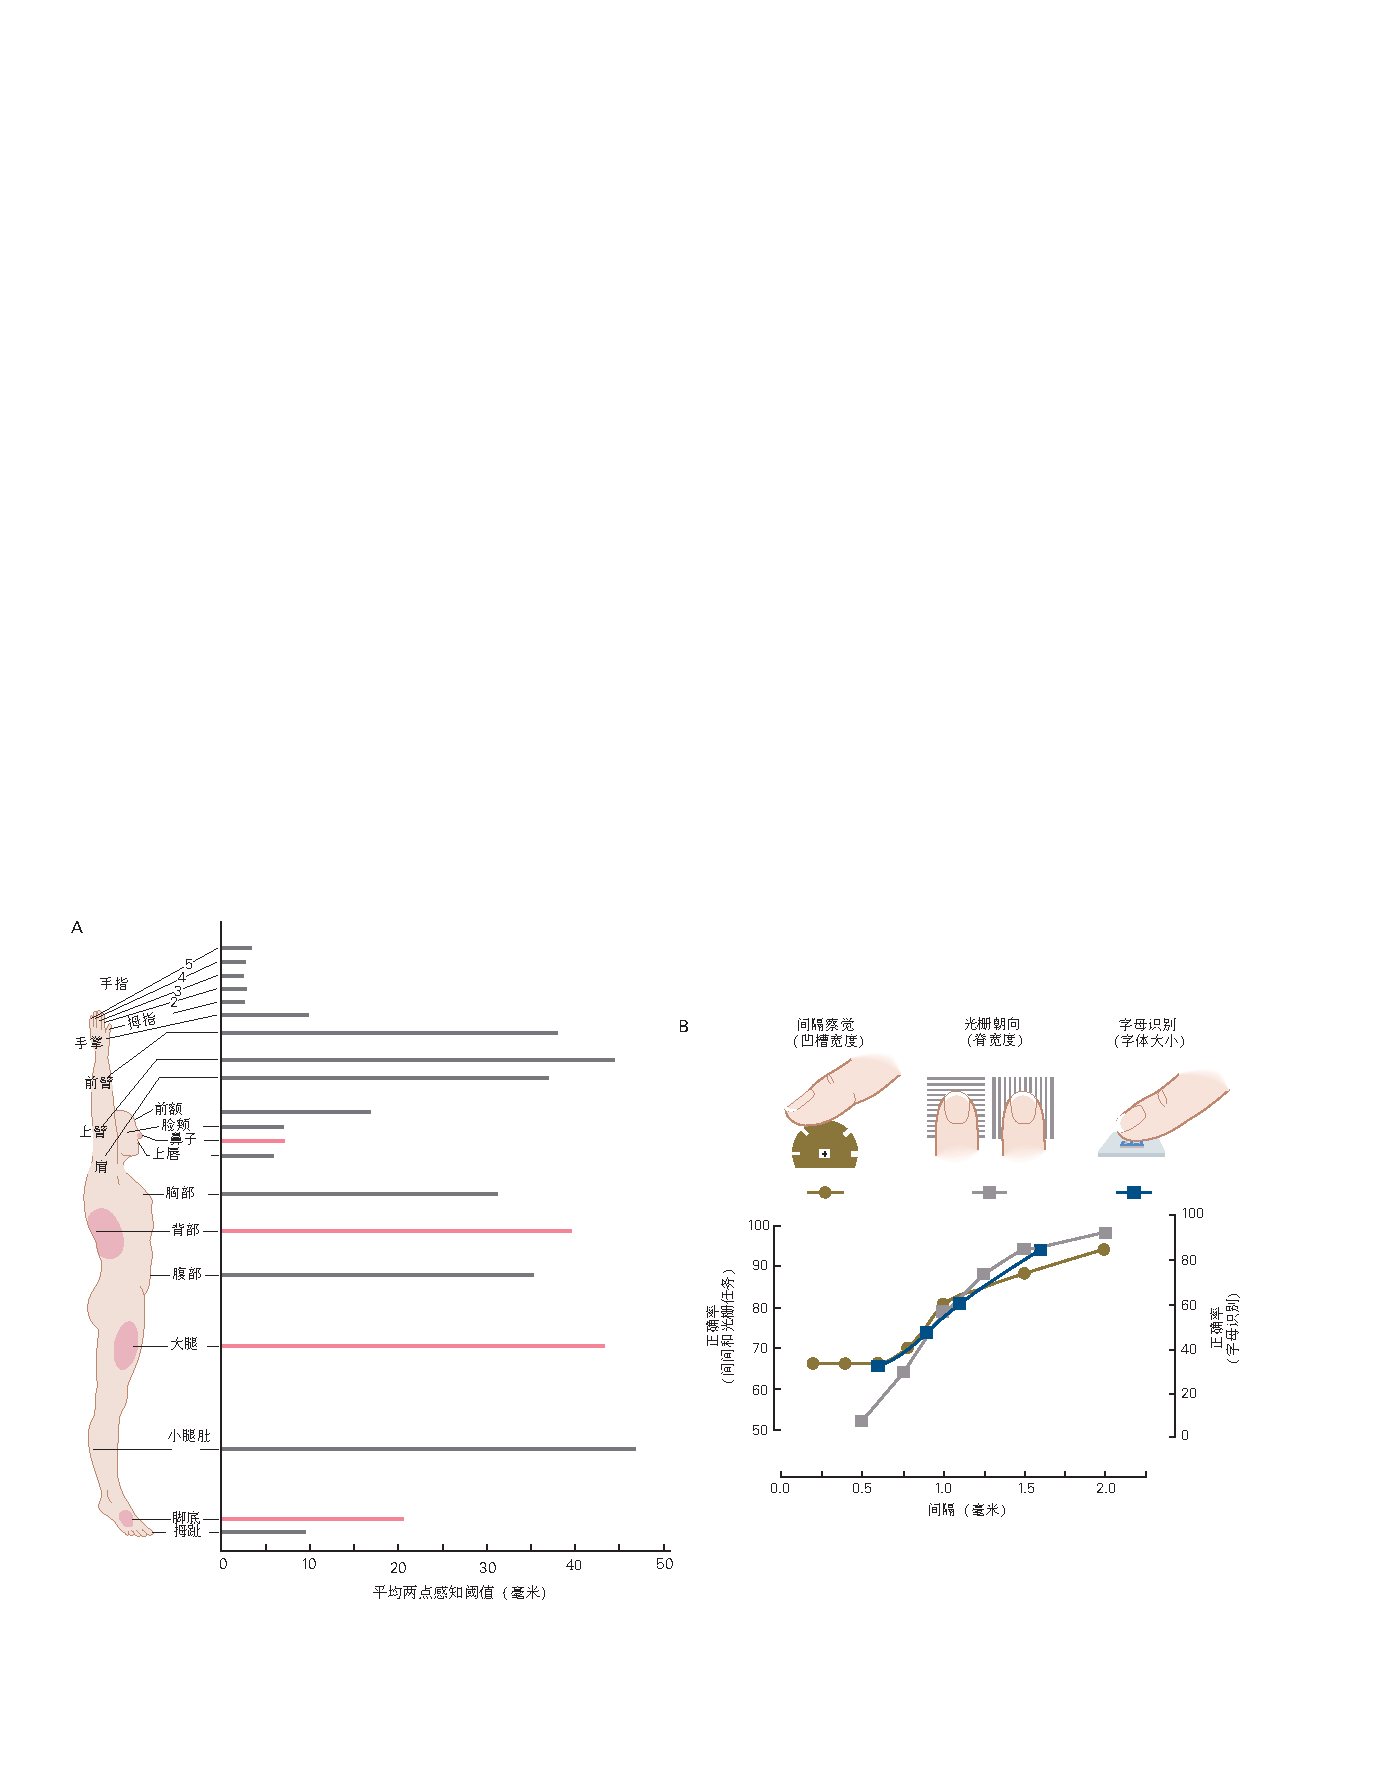
\includegraphics[width=1.0\linewidth]{chap19/fig_19_6}
	\caption{人手的触觉敏锐度在指尖最高。
		A. \textit{两点阈值}测量 2 个刺激被分辨为不同的最小距离。
		该距离因身体不同部位而异;
		它在手指上约为 2 毫米,但在手掌上可达 10 毫米,在手臂、大腿和背部可达 40 毫米。
		不同身体部位的平均两点感知阈值,由条形图中的粉红色线条表示,与身体上相应粉红色区域的平均感受野直径相匹配。
		指尖、嘴唇和舌头具有最大的辨别能力,它们具有最小的感受野\cite{weinstein1968intensive}。
		B. 空间敏锐度是在心理物理学实验中通过让被蒙住眼睛的受试者触摸各种纹理表面来测量的。
		如图所示,受试者被要求确定轮子的表面是光滑的还是有缝隙,光栅的脊线是横跨手指还是平行于手指的长轴,或者哪些字母出现在凸起的字体上活版印刷。
		触觉敏锐度阈值定义为产生 75\% 正确性能的凹槽宽度、脊宽度或字体大小(在偶然和完美准确度之间可检测到的中间值)。
		在每个测试中,人类指尖的阈值间距为 1.0 毫米\cite{johnson1981tactile}。}
	\label{fig:19_6}
\end{figure}


当我们抓取或触摸一个物体时,我们可以辨别其表面分离的特征,相隔小至 0.5 毫米。
如图~\ref{fig:19_6}B~所示,人类能够区分具有极窄的槽峰间隔的光栅的水平和垂直方向。
长边,如光栅的槽峰,在同时刺激感受野中的多个感觉末梢时,会引起\textit{快适应1型}和\textit{慢适应1型}传入神经元更强烈的响应,强调了多传感器感受野对触觉信息处理的重要性。
\textit{罗兰$\cdot$约翰逊}和\textit{安德鲁$\cdot$普鲁斯钦斯基}最近发现,当边缘接触多个感觉末梢时,\textit{快适应1型}和\textit{慢适应1型}纤维对其响应更强烈,使这些传入神经元能够区分垂直、水平或倾斜方向。


女性的触觉敏锐度略高于男性,并且在手指之间存在差异,但在手之间没有差异;
性别差异主要与女性乳头脊直径较小以及由此导致的每平方厘米皮肤\textit{慢适应1型}纤维密度更高有关。
远端指尖垫的敏感度最高;
空间敏感度从食指到小指逐渐下降,并在靠近远端指尖垫的位置迅速下降。
小指远端指尖垫的触觉空间分辨率较差,比手掌粗糙 6 到 8 倍。


盲人使用\textit{慢适应1型}和\textit{快适应1型}纤维的精细空间敏感度来阅读盲文。
盲文字母将字母表示为简单的圆点图案,易于触摸区分。
盲人通过手指在圆点图案上移动来阅读盲文。
这种手部运动增强了点产生的感觉。
由于盲文点之间的间距约为 3 毫米,该距离大于\textit{慢适应1型}纤维的感受野直径,因此每个点刺激一组不同的\textit{慢适应1型}纤维。
如图~\ref{fig:19_7}~所示,当一个点进入它的感受野时,\textit{慢适应1型}纤维会发出一连串动作电位,而一旦该点离开感受野,它就会停止活动。
同步发射的一组特定的\textit{慢适应1型}纤维信号指示了盲文点的空间排列。
\textit{快适应1型}纤维也可以区分点图案,增强了\textit{慢适应1型}纤维提供的信号。


\begin{figure}[htbp]
	\centering
	\includegraphics[width=1.0\linewidth]{chap19/fig_19_7}
	\caption{触觉受体对手指扫描的盲文点的响应。
		字母 A 到 R 的盲文符号安装在一个鼓上,该鼓在人类受试者的指尖上反复旋转。
		每次旋转后,鼓向上移动,以便在手指上扫描另一部分符号。
		放置在该受试者正中神经中的微电极记录了支配指尖的机械感受纤维的响应。
		当盲文符号在感受野上移动时,神经纤维释放的动作电位在这些记录中用小点表示; 每个水平行的点代表纤维对鼓的单次旋转的响应。
		\textit{慢适应1型}受体记录了盲文符号最清晰的图像,用一系列动作电位代表每个盲文点,当盲文符号之间的空间不提供刺激时,它们就会变得安静。
		\textit{快适应1型}受体提供盲文符号的模糊图像,因为它们的感受域更大,但单个点图案仍然可以识别。 
		\textit{快适应2型}和\textit{慢适应2型}2受体都不能编码盲文图案的空间特征,因为它们的感受野大于点间距。
		\textit{快适应2型}纤维的高放电率反映了\textit{环层小体}对振动的敏锐敏感性\cite{phillips1990representation}。}
	\label{fig:19_7}
\end{figure}


尽管\textit{环层小体}(\textit{快适应2型}纤维)对扫描皮肤上的盲文点有响应,但它们的脉冲序列并不反映盲文图案中点的周期性。
相反,它们传递了盲文点在皮肤上移动引起的皮肤振动信号。
\textit{斯利曼$\cdot$本斯曼}及其同事最近发现,当用这种方法测试织物等精细纹理时,\textit{快适应2型} 传入信号通过生成与这些表面特征同相的脉冲序列来发出编织物中线的周期性信号。
由于螺纹尺寸通常太小,无法以足够的幅度压入皮肤。\textit{慢适应1型}纤维对织物运动的响应较差,
尽管如此,所有 3 种类型的触觉传入神经元都有助于人类感知粗糙度和光滑度。


\begin{figure}[htbp]
	\centering
	\includegraphics[width=1.0\linewidth]{chap19/fig_19_8}
	\caption{\textit{快适应2型}纤维具有最低的振动阈值。
		振动是由皮肤的正弦波刺激产生的感觉,如电动机的嗡嗡声、乐器的弦或神经系统检查中使用的音叉。
		A. 1. \textit{环层小体}由包裹\textit{快适应2型}纤维末端的同心、充满液体的结缔组织薄片组成。 这种结构特别适合运动检测。
		\textit{快适应2型}纤维中的感觉转导发生在与胶囊内层相连的拉伸敏感阳离子通道中。
		2. 当对皮肤施加稳定的压力时,\textit{快适应2型}纤维会在刺激开始和结束时爆发。
		作为对正弦刺激(振动)的响应,纤维会定期放电,这样每个动作电位都会发出一个刺激周期的信号。
		我们将振动视为有节奏地重复的事件,是由于同时激活许多 \textit{快适应2型}单元而产生的,这些单元同步发射\cite{talbot1968sense}。
		B. 1. 振动检测的心理物理阈值取决于刺激频率。
		如图所示,人类在抓取大物体时可以检测到 200 赫兹时小至 30 纳米的振动;
		阈值在其他频率和使用小探头测试时更高\cite{brisben1999detection}。
		2. 人类的振动阈值,通过压入皮肤的小探针尖端测量,与每个频率范围内最敏感的触摸纤维的阈值相匹配。 
		每种类型的机械受体纤维对特定频率范围最敏感。
		\textit{慢适应1型}纤维是 5 赫兹以下最敏感的群体,\textit{快适应1型}纤维在 10 赫兹和 50 赫兹之间,\textit{快适应2型}纤维在 50 赫兹和 400 赫兹以上\cite{mountcastle1972detection,johansson1982responses}。}
	\label{fig:19_8}
\end{figure}



\subsection{慢适应纤维检测物体的压力和形状}

\textit{慢适应1型}和\textit{慢适应2型}纤维最重要的功能是它们能够传递皮肤变形和压力信号。
\textit{慢适应1型}受体对边缘、拐角、点和曲率的敏感性提供了有关物体的柔软性、形状、大小和表面纹理的信息。
当我们触摸到一个物体时,如果它使皮肤凹陷,我们会认为它是坚硬或刚性的;如果我们使它变形,我们会认为它是软的。


矛盾的是,随着物体尺寸和直径的增加,其表面曲率会减小。
单个\textit{慢适应1型}纤维的响应变得较弱,由此产生的感觉不那么明显。
例如,将铅笔尖压入皮肤 1 毫米,感觉尖锐、令人不快,并且在接触点高度局部化,而将橡皮擦压入皮肤 1 毫米则感觉迟钝且较广泛。
而压在指垫上的平面产生的感觉最弱。


要理解为什么这些物体会引起不同的感觉,我们需要考虑触摸皮肤时发生的物理事件。
当铅笔尖压在皮肤上时,它会在接触点处使表面凹陷,并在周围区域(半径约 4 毫米)形成一个浅而倾斜的盆地。
虽然压痕力集中在中心,但周围区域也受到局部拉伸的影响,称为拉伸应变。
位于皮肤中心和周围“山坡”的\textit{慢适应1型}受体受到刺激,产生与局部拉伸程度成比例的脉冲序列。


如果将第二个探针靠近第一个探针按压,则会刺激更多的\textit{慢适应1型}纤维,但每根纤维的神经响应都会减弱,因为移动皮肤所需的力被分摊到 2 个探针之间。
\textit{肯$\cdot$约翰逊}和他的同事已经证明,随着在感受野中添加更多的探针,每个感觉末端的响应强度会逐渐变弱,因为皮肤上的位移力分布在整个接触区。
因此,皮肤力学造成了“少即是多”的情况。
单个\textit{慢适应1型}纤维对小物体的响应比对大物体的响应更强烈,因为使皮肤凹陷的力集中在一个小接触点上。
以这种方式,每个\textit{慢适应1型}纤维在其感受野内集成了局部的皮肤凹陷轮廓。


\textit{慢适应1型}受体对皮肤局部应变的敏感性使它们能够检测到边缘,即物体曲率突然变化的地方。
当手指触摸边缘时,\textit{慢适应1型}的激活率比触摸平面时高出许多倍,因为物体边界施加的力会使皮肤不对称地位移,超出边缘以及在边缘上。
这种不对称的力分布增强了沿物体边缘的感受野的响应。
由于边缘通常被认为是锋利的,我们倾向于在平坦或轻微弯曲的表面上而不是通过边缘来抓住物体。


内嵌于\textit{鲁菲尼终末器}的\textit{慢适应2型}纤维对皮肤拉伸的响应比对压痕的响应更强烈,因为它们的解剖学位置位于手掌皱襞或手指关节处。
它们提供了有关用整只手抓握大型物体的形状信息,即“握力抓握”,在这种情况下,物体被压在手掌上。


\textit{慢适应2型}系统可能在立体感知(仅通过触摸来识别三维物体)以及其他以皮肤拉伸为主要线索的感知任务中发挥核心作用。
\textit{贝诺尼$\cdot$爱丁}表明,\textit{慢适应2型}神经对手背上的\textit{毛发皮肤}的感知手形和手指位置起着重要作用。
\textit{慢适应2型}纤维通过检测指关节上的皮肤拉伸或手指之间的网状组织来帮助感知手指关节角度。
如图~\ref{fig:19_5}A~底部面板所示,这些关节附近的\textit{鲁菲尼终末器}彼此对齐,以便随着手指朝特定方向移动时刺激不同的受体组。
以这种方式,\textit{慢适应2型}系统提供了整个手部皮肤拉伸的神经表征,而非外部感知功能。


当手空着时,\textit{慢适应2型}纤维还提供有关手部形状和手指运动的本体感觉信息。
如果手指完全伸展和外展,我们会感觉到手掌和近端指骨的拉伸,因为\textit{光滑皮肤}被压平了。
同样,如果手指完全屈曲,形成拳头,我们会感觉到手背皮肤的拉伸,尤其是在掌指关节和近端指间关节上。
人类利用这种本体感觉信息来预先调整手部形状,以有效地抓取物体,将手指张开到足够大的程度以清除物体,并熟练地抓住它而不用太大力。



\subsection{快适应纤维检测运动和振动}

振动感测试是神经学检查的重要组成部分。
如图~\ref{fig:19_8}A2~所示,用以特定频率振动的音叉触摸皮肤会引起周期性的嗡嗡感,因为大多数触觉受体会同步发射与刺激频率相同的周期性动作电位序列。
振动感是动态触觉敏感的有用指标,特别是在局部神经损伤的情况下。


\textit{快适应2型}受体,即\textit{环层小体},是体感系统中最敏感的机械受体。
如图~\ref{fig:19_8}B2~所示,它对高频(30-500 赫兹)的振动刺激非常敏感,可以在纳米级别检测到 250 赫兹的振动。
\textit{环层小体}能够过滤和放大高频振动的能力使我们能够感受到手中工具工作表面的情况,就好像我们的手指本身正在触摸工具下的物体一样。
临床医生利用这种敏感度将针插入血管中,并探测组织的硬度。
汽车修理工利用振动感将扳手定位在看不见的螺栓上。
我们可以在黑暗中书写,因为我们能感觉到钢笔接触纸张时的振动,并将摩擦力从粗糙的表面传递到我们的手指。


如图~\ref{fig:19_8}B2~所示,尽管\textit{环层小体}对于大于 40 赫兹的频率具有最低的振动阈值,但更高振幅的振动刺激也会激发\textit{慢适应1型}和\textit{快适应1型}纤维,即使它们产生的的脉冲序列相对于\textit{环层小体}受体而言更弱。
图\ref{fig:19_9}A 说明了 15 种不同周围神经纤维在 20 赫兹下以弱、中等和高振幅刺激的激发放电模式。
尽管这些纤维对振动的敏感度不同,但它们的脉冲序列具有一些共同的重要特征。
首先,每个神经元在振动周期的特定阶段放电,通常是当探针压入皮肤时,并且其脉冲相位模式复制了振动频率:
当以 20 赫兹刺激时,脉冲序列以大约 50 毫秒的间隔重复出现。
脉冲序列的模式得到进一步加强,因为纤维群体同步发射,使得频率信息由于突触整合而在中央得以保留。


\begin{figure}[htbp]
	\centering
	\includegraphics[width=1.0\linewidth]{chap19/fig_19_9}
	\caption{超阈值振动激活多类触觉受体。 
		A. 从猕猴的 15 种不同体感纤维中记录的脉冲序列的光栅,这些体感纤维受到振幅为 35(左)、130(中)和 250 微米(右)的 20 赫兹振动刺激的刺激。
		交替的阴影和白色带表示个体\textit{慢适应1型}、\textit{快适应1型}和\textit{快适应2型}触摸纤维对同一刺激的 5 次呈现的响应。
		神经响应被分组为一个或多个脉冲的爆发,这些脉冲与每个振动周期的压痕阶段同步发生。
		每根纤维中每个周期的脉冲总数与振动幅度相关; 这个群体发射的脉冲总数也反映了振动幅度。
		尽管单个神经元的响应强度不同,但每条触摸纤维的脉冲序列在每次试验中都非常相似,并且在神经元之间同步发生\cite{muniak2007neural}。
		B. \textit{初级躯体感觉皮层}对 20 赫兹振动的响应。
		猕猴\textit{初级躯体感觉皮层}区域 3b(顶部)的 2 个神经元和区域 1(底部)的 2 个神经元中诱发的脉冲序列光栅。
		阴影区域表示振动刺激的周期。
		与周围神经一样,\textit{初级躯体感觉皮层}神经元对低频振动作出响应,脉冲群与刺激率同相。
		请注意,脉冲序列因试验而异,并且在区域 1 中的周期性低于区域 3b 中的周期性。
		与\textit{初级躯体感觉皮层}相比,\textit{次级躯体感觉皮层}(参见图~\ref{fig:19_21})的放电周期甚至更不明显\cite{salinas2000periodicity}。}
	\label{fig:19_9}
\end{figure}


随着刺激幅度的增加,每次爆发的脉冲序列数也增加,使得每根纤维能够将振动频率和强度的信号进行多路复用:
频率信息由脉冲序列的时间模式传递,而振动幅度则由每根纤维每秒发射的总脉冲数以及激活得纤维群体的总脉冲输出编码。
最后,请注意,每个神经元的脉冲序列在每个条件的试验中在时间上和脉冲计数上都非常相似,这表明触觉传入纤维提供的感觉信号具有很高的可靠性。 
触觉编码的这种可靠性和可预测性使得振动成为评估触觉的一种特别有用的技术。



\subsection{慢适应和快适应纤维对抓握控制都很重要}

除了感知物体的物理特性外,触觉受体还提供有关熟练动作中手部动作的重要信息。
\textit{罗兰$\cdot$约翰逊}和\textit{格伦$\cdot$韦斯特林}利用微神经图法确定了触觉受体在物体被受握住时的作用。。
通过在正中神经中放置微电极,当手指初次接触物体时,以及当物体被拇指和食指夹住、举起、放在桌子上方、放低、并回到原位时,他们能够记录触觉纤维的放电模式。


他们发现所有 4 类触觉纤维都对抓握有响应,并且每种纤维类型都负责监测特定的功能。
在没有触觉刺激的情况下,\textit{快适应1型}、\textit{快适应2型}和\textit{慢适应1型}纤维通常处于静默状态。
如图~\ref{fig:19_10}~所示,当物体首次被触碰时,它们会检测到接触。
\textit{慢适应1型}纤维负责发出每个手指施加的握力大小信号,\textit{快适应1型}纤维负责感知握力施加的速度。
\textit{快适应2型}纤维负责检测物体被从桌子上提起到放回时通过物体传递的微小冲击波。
由于这些振动,我们能够知道物体何时与桌面接触,因此可以在不看物体的情况下操纵物体。
在抓握完成后,\textit{快适应1型}和\textit{快适应2型}纤维会停止响应。
\textit{慢适应2型}纤维在抓握或释放物体时发出手指弯曲或伸展的信号,从而在这些动作进行时监测手部姿势。


\begin{figure}[htbp]
	\centering
	\includegraphics[width=1.0\linewidth]{chap19/fig_19_10}
	\caption{在抓取和举起过程中来自手的感觉信息\cite{johansson1996sensory}。
		A. 受试者在拇指和指尖之间抓住并提起一块木块,将其放在桌子上方,然后将其放回静止位置。
		法向(抓握)力将物体固定在手中,切向(负载)力克服重力。
		握力适应物体的表面纹理和重量。
		B. 夹持力和负载力由物体中的传感器监控。
		这些力在与物体接触后协调,在升力开始时稳定,并在物体返回到桌子后一致放松。
		C. 所有 4 个机械受体都检测到手与物体的接触,但随着任务的进行,每个都监测动作的不同方面。
		\textit{慢适应1型}纤维编码握力,\textit{慢适应2型}纤维编码手部姿势。
		\textit{快适应1型}纤维对手在物体上施加力和移动的速率进行编码。
		\textit{快适应2型}纤维在每个任务阶段感知物体的振动:
		手部接触、抬起、桌面接触和松开抓握。}
	\label{fig:19_10}
\end{figure}


手部传来的关于物体形状、大小和纹理的信号是在抓握过程中施加力量的重要因素。
\textit{约翰逊}和他的同事发现,我们能够灵敏地举起和操纵物体(握力刚好超过导致明显滑动的力),并且握力会自动调整以补偿手指和物体表面之间摩擦系数的差异。
受试者根据\textit{慢适应1型}和\textit{快适应1型}传入神经提供的触觉信息来预测抓握和举起物体所需的力,并根据这些信息调整力量大小。
表面光滑的物体比表面粗糙的物体抓握得更牢固,这些属性由\textit{快适应1型}感觉神经元在手初次接触物体时编码。
触觉信息在抓握中的重要性在神经损伤或手部局部麻醉的情况下尤为显著;
患者施加异常高的握力,并且手指施加的握力和负载力之间的协调性较差。


\textit{快适应1型}受体提供的信息对于监测抓握动作至关重要,它使我们能够在突然滑动时保持物体不松动。
\textit{快适应1型}纤维在稳定抓握过程中通常保持沉默,直到物体恢复静止并松开抓握。
然而,如果物体突然变得沉重或被外力颠簸,并开始从手中滑落,\textit{快适应1型}纤维会对物体的微小切向滑动运动作出响应而发出响应。
这种\textit{快适应1型}活动的最终结果是:运动皮层发出的信号会增加抓握力。



\section{触觉信息在中央触摸系统中处理}

手部感觉传入纤维通过\textit{正中神经}、\textit{尺神经}和\textit{浅桡神经}将触觉和其他体感信息传递到中枢神经系统。
这些神经终止于同侧的 C6 至 T1 脊髓节段;
如图~\ref{fig:19_11}~所示,这些纤维的其他分支通过同侧脊髓背柱直接投射到延髓,在那里它们与\textit{楔形核}中的神经元建立突触连接,楔形核是背柱核的外侧部分。


\begin{figure}[htbp]
	\centering
	\includegraphics[width=0.99\linewidth]{chap19/fig_19_11}
	\caption{来自四肢和躯干的体感信息通过两条上行通路传递到\textit{丘脑}和大脑皮层。
		沿着从脊髓到大脑的神经轴的脑切片说明了将体感信息传递到大脑皮层的两条主要通路的解剖结构。
		这两条通路在到达\textit{脑桥之前}是\textit{分开}的,它们在那里并列。
		背柱,即内侧丘系系统(橙色)。
		触摸和肢体本体感觉信号通过大直径有髓神经纤维传递到脊髓和脑干,并在该系统中传递到丘脑。
		在脊髓中,用于触觉和本体感觉的纤维分开,一个分支进入同侧脊髓灰质,另一个在同侧背柱中上行到\textit{延髓}。
		来自背柱核神经元的二级纤维在\textit{延髓}中穿过中线并在对侧内侧丘系中上行至丘脑,在那里它们终止于外侧和内侧腹侧后核。
		这些核中的丘脑神经元将触觉和本体感受信息传递给初级体感皮层。 前外侧系统(棕色)。
		疼痛、瘙痒、温度和内脏信息通过终止于同侧背角的小直径有髓和无髓纤维传递到脊髓。
		该信息由脊髓内的神经元通过中线传递,并传递到对侧前外侧系统中的脑干和丘脑。
		终止于脑干的前外侧纤维组成脊髓网状束和脊髓中脑束; 剩余的前外侧纤维形成脊髓丘脑束。}
	\label{fig:19_11}
\end{figure}



\subsection{脊髓、脑干和丘脑回路分离触觉和本体感觉}

脊髓背柱中的纤维和背柱核中的神经元以拓扑学方式组织,上半身(包括手)在楔形束和核的外侧表示,下半身在细束和核的内侧表示。
在这些区域,触觉和本体感觉的感觉亚模式也在功能上分离,因为单个脊髓和脑干神经元接收来自单一类型的传入神经元的突触输入,而不同类型的神经元在空间上分离。 
背柱核的前 1/3 主要由处理肌肉传入神经信息的神经元组成;触觉输入主要在尾部更占优势。
感觉模式的分离是主要体感皮层投射通路的一致特征。


背柱核中的神经元通过脑干中线将其轴突投射到形成中间束的对侧,中间束时一个突出的纤维束,通过脑桥和中脑将来自对侧身体的触觉和本体感觉信息传输到丘脑。
由于感觉纤维的交叉,大脑的左侧接收来自身体右侧的机械受体的体感输入,反之亦然。
在传递过程中,丘脑内部和中间束中的身体的拓扑表征发生反转;
身体的拓扑图在中间显示面部,下半身显示在外侧,上半身和手部则介于两者之间。


来自手部和身体其他部位的触觉和本体感觉信息在丘脑的不同亚核中进行处理。
四肢和躯干的触觉信号通过中间束发送到\textit{腹后外侧核},而来自面部和口腔的触觉信号则传送到\textit{腹后内侧核}。
来自肌肉和关节(包括手部)的本体感觉信息被传输到\textit{腹后上核}。
这些核将它们的输出发送到大脑皮层顶叶的不同亚区。 
\textit{腹后外侧核}和\textit{腹后内侧核}主要将皮肤信息传递到\textit{初级躯体感觉皮层}的 3b 区,而\textit{腹后上核}主要将本体感受信息传递到 3a 区。



\subsection{体感皮层被组织成功能专门化的柱状体}

有意识的触觉感知被认为起源于大脑皮层。
触觉信息通过顶叶海马后回的\textit{初级体感皮层}进入大脑皮层。
如图~\ref{fig:19_12}~所示,\textit{初级体感皮层}包括 4 个细胞结构区域:布罗德曼区域 3a、3b、1 和 2。
这些区域相互关联,使得\textit{初级体感皮层}中的感觉信息处理涉及串行和并行处理。


\begin{figure}[htbp]
	\centering
	\includegraphics[width=1.0\linewidth]{chap19/fig_19_12}
	\caption{人脑中大脑皮层的体感区。
		A. 皮层的体感区域位于顶叶,由 3 个主要部分组成。
		\textit{初级躯体感觉皮层}形成顶叶的前部。
		它从中央沟底部开始延伸到整个中央后回,向后延伸至中央后沟,并进入半球内侧壁至扣带回(未显示)。
		\textit{初级躯体感觉皮层}包括 4 个不同的细胞构造区域:\textit{布罗德曼} 3a、3b、1 和 2 区。
		\textit{次级躯体感觉皮层}位于外侧沟(外侧裂)上岸和顶叶盖上;
		它覆盖\textit{布罗德曼} 43 区。
		后顶叶皮层围绕半球外侧表面的顶内沟,从中央后沟延伸至顶枕沟,并在内侧延伸至楔前叶。
		上顶叶小叶(\textit{布罗德曼}  5 和 7 区)是一个体感区;
		下顶叶小叶(区域 39 和 40)接收体感和视觉输入。
		B. 中央后回的冠状切面说明了\textit{初级躯体感觉皮层}、\textit{次级躯体感觉皮层}和初级运动皮层(区域 4)的解剖关系。
		\textit{次级躯体感觉皮层}与\textit{初级躯体感觉皮层}中的区域 2 相邻,并沿着外侧沟的上岸向内侧延伸至岛叶皮层。
		初级运动皮层位于中央沟前壁内 3a 区的嘴侧。}
	\label{fig:19_12}
\end{figure}


在对大脑皮层进行的一系列开创性研究中,\textit{弗农$\cdot$芒卡斯尔}发现\textit{初级体感皮层}是由垂直的柱状结构或板块组成的。
如图~\ref{fig:19_13}~所示,每个柱状结构宽 300 至 600 微米,横跨从皮层表面到白质的所有 6 个皮层。
柱状结构内的神经元接收来自同一局部皮肤区域的输入,并对同一类或多类触觉受体做出响应。
因此,柱状结构包含新皮层的基本功能模块;
它提供了一个解剖结构,用于组织感觉输入以传达有关位置和形态的相关信息。


\begin{figure}[htbp]
	\centering
	\includegraphics[width=0.75\linewidth]{chap19/fig_19_13}
	\caption{躯体感觉皮层柱内神经回路的组织。
		来自皮肤或深层组织的感觉输入被组织成从大脑表面延伸到白质的神经元柱。
		每一柱主要在第四层接收来自身体一部分的丘脑输入。
		IV 层中的兴奋性神经元将其轴突垂直送向皮层表面,接触 II 层和 III 层(颗粒上层)中\textit{锥体神经元}的树突以及颗粒下层(V 层和 VI 层)中锥体细胞的顶端树突。
		以这种方式,来自身体部位(例如手指)的触觉信息垂直分布在一列神经元内。}
	\label{fig:19_13}
\end{figure}


皮层的柱状组织是内在皮层回路、丘脑皮层轴突的投射模式和皮层发育过程中神经原迁移路径的直接结果。
柱状结构内连接的模式呈垂直方向,与皮层表面垂直。
丘脑皮层轴突主要终止于第 IV 层的星状细胞簇,其轴突垂直投射到皮层表面,以及星形\textit{锥体细胞}。
因此,丘脑皮层输入被中继到受第 IV 层细胞轴突接触的\textit{锥体细胞}的窄柱中。
如图~\ref{fig:19_14}~所示,皮层\textit{锥体细胞}的顶树突和轴突在其他皮层中也主要是垂直方向排列的,与丘脑皮层轴突和星形细胞轴突平行。
这使得相同的信息可以由整个皮层厚度的一列神经元处理。


\begin{figure}[htbp]
	\centering
	\includegraphics[width=1.0\linewidth]{chap19/fig_19_14}
	\caption{体感皮层的柱状组织。
		6 层中的皮层兴奋性神经元具有独特的金字塔型形状,具有大细胞体、一个垂直向皮层表面突出并在更表层分枝的单个顶端树突,以及靠近细胞体分枝的多个基底树突。
		\textit{锥体神经元}在大小、基因表达模式、顶端树突的长度和厚度以及轴突的投射目标方面存在差异。
		所有这些神经元都在大脑皮层内的目标上形成突触。
		此外,V 层的\textit{锥体神经元}皮层下投射到脊髓、脑干、中脑和基底神经节。
		第六层的皮层丘脑神经元投射回传入丘脑核,为该柱提供感觉输入。
		第四层的多刺星状神经元是唯一显示的不是\textit{锥体神经元}的兴奋性细胞\cite{oberlaender2012cell}。}
	\label{fig:19_14}
\end{figure}


\textit{锥体神经元}是体感皮层的主要兴奋性神经元类,
约占\textit{初级体感皮层}神经元的 80\% 。 
如图~\ref{fig:19_14}~所示,每个皮层的\textit{锥体神经元}都投射到特定的靶点。
横向的循环连接将同一列或相邻列的\textit{锥体神经元}连接起来,使得它们在被相同刺激同时激活时共享信息。
第 II 层和第 III 层中的神经元也会将信息投射到同一列中的第 V 层,投射到同侧更高级别的皮层区域,并投射到相反半球的镜像位置。
这些向更高级别的皮层区域的前馈连接允许进行复杂的信号整合,正如本章后面描述的那样。


第 V 层中的\textit{锥体神经元}为每个柱状体提供主要的输出。
它们接收来自同一柱状体或相邻柱状体中第 II 层和第 III 层神经元的兴奋性输入,以及稀疏的丘脑皮层输入。
如图~\ref{fig:19_17}C~所示,第 V 层(V-A 层)浅部的神经元向高阶皮层区域的 IV 层发送双侧前馈输出,并向纹状体发送。
第 V 层(V-B 层)深处的神经元投射到基底神经节、上丘、脑桥和其他脑干核团、脊髓和背柱核团等皮层下结构。
第Ⅵ层的神经元投射到局部皮层神经元,并返回丘脑,特别是投射到为该柱状体提供输入的腹后核区域。


\begin{figure}[htbp]
	\centering
	\includegraphics[width=0.5\linewidth]{chap19/fig_19_17}
	\caption{\textit{初级躯体感觉皮层}的手部区域。 
		A. 这个通过手部表示的矢状切面说明了人脑中\textit{初级躯体感觉皮层}的 4 个子区域(区域 3a、3b、1 和 2)以及相邻的初级运动皮层(区域 4)和后顶叶皮层(区域 5)。
		皮层表面上的标签表示代表各个手指的柱(D2–D5);
		向右的箭头表示大脑中的部分方向。
		4 个\textit{初级躯体感觉皮层}区域处理不同类型的体感信息,由皮层部分下方颜色匹配的矩形指示。
		区域 5 中的神经元主要响应以目标为导向的主动手部运动。
		B. 猕猴\textit{初级躯体感觉皮层}各区域神经元的典型感受野在手部图标上显示为彩色斑块。
		通过轻触皮肤或移动各个关节来勾勒出区域。
		感受野在区域 3a 和 3b 中最小,触觉信息首先进入大脑皮层,区域 1、2 和 5 中的感受野逐渐变大,反映出来自区域 3b 中的神经元的汇聚输入,这些神经元在使用手时会一起受到刺激。
		区域 5 和\textit{次级躯体感觉皮层}中的神经元通常具有双侧感受野,因为它们对双手镜像位置的触摸做出响应\cite{gardner1988somatosensory,iwamura1993rostrocaudal,iwamura1994bilateral}。
		C. 体感皮层区域之间的前馈层次连接。
		丘脑皮层和皮层连接的强度由连接这些区域的箭头粗细表示。
		丘脑中的神经元主要将其轴突发送到区域 3a 和 3b,但有些也投射到区域 1 和 2。反过来,皮层区域 3a 和 3b 中的神经元投射到区域 1 和 2。
		来自\textit{初级躯体感觉皮层} 4 个区域的信息被传递 到后顶叶皮层(区域 5)和\textit{次级躯体感觉皮层}中的神经元。
		其中许多连接是双向的。
		高阶皮层区域的神经元投射回低阶区域,特别是 I 层。\cite{felleman1991distributed}。}
	\label{fig:19_17}
\end{figure}


除了来自触觉受体的前馈信息信号外,来自高级体感皮层区域的第 II 层和第 III 层的反馈信号也被提供给较低皮层区域的第 I 层,从而调节其兴奋性。
这种反馈信号不仅来源于体感皮层区域,还来源于后顶叶皮层的感觉运动区域、额叶运动区域、边缘区域以及参与记忆形成和存储的内侧颞叶区域。
这些反馈信号被认为在认知处理(通过注意力机制)中选择感觉信息以及执行短期记忆任务方面发挥着作用。
在运动活动期间,反馈通路还能控制感觉信号。
每个柱状体内部的各种局部抑制性中间神经元负责集中柱状体的输出。



\subsection{皮层柱状体按体位图组织}

如图~\ref{fig:19_15}~所示,初级躯体感觉皮层内的柱状体是按照\textit{拓扑映射}排列的,因此在\textit{初级体感皮层}的 4 个区域中都有一个完整的躯体定位图。
如图~\ref{fig:18_13}~所示,身体的皮层图大致对应于脊髓皮节。
骶骨段位于正中部位,腰椎和胸椎段位于中心部位,颈椎段更靠外侧,而面部的三叉神经表示位于\textit{初级体感皮层}的最外侧部分。
了解大脑中的身体神经图对于定位中风或头部创伤引起的皮层损伤非常重要。


\begin{figure}[htbp]
	\centering
	\includegraphics[width=0.95\linewidth]{chap19/fig_19_15}
	\caption{初级体感皮层的每个区域都包含整个身体表面的地形神经映射\cite{nelson1980representations}。
		A. 与人脑一样,猕猴的初级体感皮层位于中央沟的尾部。
		猕猴皮层上的彩色区域对应于图~\ref{fig:19_12}~中人脑的同源布罗德曼区域。
		猕猴的第 5 区与人类的第 5 区和第 7 区同源。
		猕猴的第 7 区与人类的第 39 区和 40 区同源。
		B. 右边的平面图显示了猕猴的体感皮层沿着中央沟展开(与区域3b和1之间的边界平行的虚线)。
		该图的上部包括从半球内侧壁展开的皮层。
		身体映射是从中央后回的微电极记录中获得的。
		身体表面被映射到按脊柱皮节顺序排列的头尾带内的列。
		区域 3b 和 1 中的身体映射形成每个皮刀的远端-近端或背-腹轴的镜像。
		每个手指(D5–D1)在区域 3b 和区域 1 中沿皮层的内侧-外侧轴都有自己的表示,但来自几个相邻手指的输入汇聚在区域 2 和区域 5 的神经元的感受野中。
		C. 高度神经支配的皮肤区域的皮层放大。
		尽管躯干(紫色)比手指(红色)覆盖的皮肤面积更大,但由于手指的神经支配密度更高,对手指上的触摸做出响应的皮层柱的数量几乎是通过触摸躯干激活的数量的 3 倍。}
	\label{fig:19_15}
\end{figure}


在顶叶中,体表至少以 10 种不同的神经图形表示:
4 个在\textit{初级体感皮层}中,4 个在\textit{次级体感皮层}中,至少 2 个在后顶叶皮层中。
因此,这些区域调节触觉的不同方面。
\textit{初级体感皮层}的 3b 区和 1 区神经元处理表面纹理的细节,而区域 2 区的神经元则处理物体的大小和形状信息。
这些躯体感觉属性在\textit{次级体感皮层}和后顶叶皮层中得到进一步阐述,其中神经元分别参与物体的辨别和操纵。


躯体定位图的另一个重要特征是每个身体部位所占的大脑皮层面积。。
人脑中的身体神经图被称为“小人图”,并没有完全复制皮肤的空间地形。
相反,身体的每个部分都按照其对触觉的重要性来表示。 
某些身体区域,特别是手、足和口,占据了不成比例的大面积,而较近端的身体部分则占据相对较小的面积。
如图~\ref{fig:19_15}C~所示,在人类和猴子中,用于手指的皮层柱状体数量比用于整个躯干的要多。


分配给皮肤单位面积的皮层面积(称为皮层放大率)在不同的身体表面上相差超过一百倍。
它与神经支配密度密切相关,因此与皮肤区域中触觉受体的空间敏锐度密切相关。
在人类大脑中,皮层放大程度最大的区域(嘴唇、舌头、手指和脚趾)的触觉敏锐度阈值分别为 0.5、0.6、1.0 和 4.5 毫米。


用胡须探测环境的啮齿动物和其他哺乳动物在\textit{初级体感皮层}中有大量柱状体,称为桶状结构,它们接收来自面部单个触须的输入(文本框~\ref{box:19_2})。
桶状皮层为研究皮层电路提供了广泛使用的实验准备。



\begin{proposition}[啮齿动物须桶系统] \label{box:19_2}
	
	\quad \quad 啮齿类动物须筒系统是现代神经科学中广泛使用的动物模型。
	,大多数哺乳动物和所有灵长类动物的脸上都有特殊的触觉毛发,称为触须。
	与皮肤上的其他毛发不同,触须生长于毛囊中,毛囊由三叉神经支配,周围是充满血液的窦。
	
\end{proposition}


\begin{figure}[htbp]
	\centering
	\includegraphics[width=1.0\linewidth]{chap19/fig_19_16}
	\caption{啮齿类动物的“桶状皮层”代表了地形模式中的振颤。
		筒状皮层是啮齿类动物\textit{初级躯体感觉皮层}的一个亚区域,代表面部触须,是一种被广泛研究的用于破译皮层回路的结构。
		A. 经\textit{5-羟色氨}染色的幼年大鼠体感皮层第四层切向组织学切片。
		较暗的免疫响应斑块对应于特定身体部位的皮层表现。
		啮齿类动物体感皮层图的最大部分专门用于触须。
		B. \textit{初级躯体感觉皮层}中宏观振动表现的放大视图。
		脸上胡须的空间模式是根据动物而定的,允许每个皮层“桶”通过带有字母的行和带有相应胡须数量的弧(列)来识别。
		每个桶中的神经元对这根主要胡须的运动响应最为强烈。
		C. 沿着轴突从丘脑\textit{腹后内侧}核到\textit{初级躯体感觉皮层}的路径倾斜切割的大鼠脑切片。
		绿色荧光蛋白标记的\textit{腹后内侧}轴突通过\textit{内囊}投射到皮层下白质,并在进入皮层之前平行于软脑膜表面行进。
		轴突密集地支配第四层,在那里它们形成离散的管状体,并更稀疏和扩散地支配第五层和第六层的边界。
		比例尺=1 毫米。
		D. 皮层中管状体的地形排列与面部振动的空间排列成行(字母)和弧(数字)相匹配。}
	\label{fig:19_16}
\end{figure}



\subsection{皮层神经元的感受野整合来自邻近受体的信息}


\textit{初级躯体感觉皮层}中的神经元至少比皮肤中的触觉受体多了 3 个突触。
它们的输入代表了背柱核、丘脑和皮层本身处理过的信息。 
每个皮层神经元接收来自皮肤特定区域受体的输入,这些输入一起构成它的感受野。
我们感知到皮肤上的特定位置被触摸,是因为皮层中特定群体的神经元被激活。
这种体验可以通过在实验中对相同皮层神经元进行电刺激或光遗传学刺激来诱发。


皮层神经元的感受野比外周神经中的体感纤维的感受野大得多。
例如,支配指尖的\textit{慢适应1型}和\textit{快适应1型}纤维的感受野是皮肤上的小点(图~\ref{fig:19_5}),而接收这些输入的皮层神经元的感受野覆盖整个指尖或几个相邻的手指(图~\ref{fig:19_17}B)。
3b 区域中神经元的感受野代表了 300 到 400 根神经纤维的复合输入,通常覆盖单个指骨或掌垫。
来自\textit{慢适应1型}和\textit{快适应1型}触觉受体的输入在同一皮肤区域汇聚到 3b 区域中的共同神经元上。


高级皮层区域的感受野甚至更大,跨越在运动活动期间同时激活的皮肤功能区域。
这些区域包括几个相邻手指的指尖,或整个手指,或手指和手掌。
\textit{初级躯体感觉皮层}1  和 2 区域中的神经元涉及的信息比它们在身体上的神经支配部位更抽象。
当同时触摸多个手指时,其感受野包括多个手指的神经元会以更高的速率放电,并以这种方式发出信号,表面手中物体的大小和形状。
这些大的感受野使皮层神经元能够整合来自单个触觉受体的碎片化信息,使我们能够识别物体的整体形状。
例如,这些神经元可以区分螺丝刀的手柄和刀刃。


来自\textit{初级躯体感觉皮层}中不同感觉受体的汇聚输入也可能使单个神经元检测物体的大小和形状。
虽然区域 3b 和 1 中的神经元仅对触摸有响应,而区域 3a 中的神经元对肌肉拉伸有响应,但区域 2 中的许多神经元同时接收 2 种输入。
因此,区域 2 中的神经元可以整合有关用于抓取物体的手形、手施加的握力以及物体产生的触觉刺激的信息;
这种整合信息可能足以识别物体。


如图~\ref{fig:19_18}~所示,皮层神经元的感受野通常有一个被抑制区包围或叠加的兴奋区。
刺激兴奋区以外的皮肤区域可能会降低神经元对感受野内触觉刺激的响应。
类似地,在感受野内反复刺激也可能降低神经元的响应性,因为局部中间神经元介导的持续较长时间的抑制会降低神经通路的兴奋性。


\begin{figure}[htbp]
	\centering
	\includegraphics[width=1.0\linewidth]{chap19/fig_19_18}
	\caption{皮层神经元的兴奋性和抑制性输入的空间排列决定了哪些刺激特征由神经元编码。
		A. 初级躯体感觉皮层 3b 区的神经元在其感受野内具有重叠的兴奋区和抑制区\cite{dicarlo1998structure,sripati2006spatiotemporal}。
		B. 具有相同兴奋区和抑制区排列的 3 个突触前神经元的聚合允许神经元中的方向和定向选择性 在区域 2。
		1. 水平杆向下运动穿过突触后细胞的感受野会产生强烈的兴奋响应,因为同时接触所有 3 个突触前神经元的兴奋场。
		酒吧的向上运动强烈抑制射击,因为它首先进入所有 3 个抑制区域。
		神经元对通过兴奋场的向上运动响应不佳,因为最初的抑制比刺激持续更久。
		2. 垂直条穿过感受野的运动会引起微弱的响应,因为它同时穿过输入神经元的兴奋性和抑制性感受野。
		在此示例中无法区分向左或向右的运动。}
	\label{fig:19_18}
\end{figure}


抑制性感受野通过背柱核、丘脑和皮层本身中的中间神经元的前馈连接和反馈连接产生,它们限制了兴奋的传播。
由一个回路中强烈活动产生的抑制作用会减少附近仅被弱兴奋的神经元输出。
抑制网络确保传递几种竞争响应中最强的一种,从而允许赢者通吃策略。
当大量触觉神经元受到刺激时,这些回路可以防止纹理等触觉细节模糊。
此外,大脑中的高层中枢会使用抑制回路,通过抑制不需要的、分散注意力的输入,在熟练的任务中使用手时,将注意力集中在相关信息上。


感受野在皮肤上的大小和位置不是永久固定的,而是可以根据感觉神经的经验或损伤来改变(第~\ref{chap:chap53}~章)。
皮层感受野似乎在发育过程中形成,并通过同步激活输入通路来维持。
如果周围神经受伤或被横切,其皮层投射目标会从通常被抑制网络抑制效率较低的感觉输入中获得新的感受野。
或从保留神经支配的邻近皮肤区域新形成的连接中获得新的感受野。
同样,通过重复练习对传入通路的广泛刺激可能会加强突触输入,从而改善知觉,提高性能。




\section{触摸信息在连续的中央突触中变得越来越抽象}

如图~\ref{fig:19_17}C~所示,体感信息从\textit{初级躯体感觉皮层}的 4 个区域并行传递到皮层中的更高中枢,例如\textit{次级躯体感觉皮层}、后顶叶皮层和初级运动皮层。
随着信息流向更高阶的皮层区域,需要特定的刺激模式组合来激活单个神经元。


如图~\ref{fig:19_19}~所示,来自邻近神经元的信号在更高的皮层区域中组合,以识别物体的全局特性,例如它们在手上的方向或运动方向。
一般来说,较高皮层区域的皮层神经元关注与其感受野中刺激位置无关的感觉特征,抽象出特定类别刺激的共同物体特性。



\begin{figure}[htbp]
	\centering
	\includegraphics[width=1.0\linewidth]{chap19/fig_19_19}
	\caption{区域 2 中的神经元编码复杂的触觉信息。 
		这些神经元对探针穿过感受野的运动做出响应,但不会接触到单个点。
		下面的迹线表示向上和向下偏转的运动方向\cite{warren1986objective}。
		A. 运动敏感神经元对在各个方向抚摸皮肤做出响应。
		B. 方向敏感的神经元对朝向手掌尺侧的运动响应强烈,但对相反方向的运动没有响应。
		对远端或近端运动的响应较弱。
		C. 方向敏感的神经元对横跨手指(尺桡)的运动比对沿手指(远端-近端)的运动响应更好,但不区分尺骨与桡骨或近端与远端方向。}
	\label{fig:19_19}
\end{figure}


由于突触感受野的空间排列,皮层神经元能够检测边缘的方向或运动方向。
兴奋性突触神经元的感受野通常沿着一个共同的轴线排列,生成后突触神经元的\textit{偏好方向}。
此外,如图~\ref{fig:19_18}B~所示,抑制性突触前神经元的感受野位于兴奋区的一侧,增强了后突触神经元的方向选择性和运动方向性。



\subsection{认知触觉由次级躯体感觉皮层中的神经元介导}

\textit{初级躯体感觉皮层}神经元对触摸的响应主要取决于神经元感受野内的输入。
这种前馈通路通常被描述为自下而上的过程,因为外围的受体是\textit{初级躯体感觉皮层}神经元兴奋的主要来源。


高阶体感区域不仅从外周受体接收信息,而且还受到自上而下的认知过程的强烈影响,例如目标设定和注意力调节。
如图~\ref{fig:17_13}~所示,从各种研究中获得的数据(猴子的单神经元研究、人类神经影像学研究以及高阶体感区域受损患者的临床观察)表明顶叶的腹侧和背侧区域在触觉系统中起着互补的作用类似于视觉系统的\textit{内容通路}和\textit{空间通路}。


如图~\ref{fig:19_12}B~和图~\ref{fig:19_20}B~所示,\textit{次级躯体感觉皮层}位于人类和猴子外侧沟的上岸和相邻的顶叶盖。
与\textit{初级躯体感觉皮层}一样,\textit{次级躯体感觉皮层}包含 4 个不同的解剖学子区域,具有单独的身体映射。
由\textit{次级躯体感觉皮层}本身和相邻的顶叶腹侧区域组成的中央区域接收来自区域 3b 和 1 的主要输入,主要是来自手和面部的触觉信息。
如图~\ref{fig:19_20}~所示,一个更靠近头端的区域(即顶叶腹侧区域)从区域 3a 接收有关主动手部运动的信息以及来自区域 3b 和 1 的触觉信息。
如图~\ref{fig:19_12}A~所示,外侧沟最尾端的体感区域延伸到顶叶盖。
该区域紧靠后顶叶皮层,并在整合物体的体感和视觉特性方面发挥作用。


\begin{figure}[htbp]
	\centering
	\includegraphics[width=0.85\linewidth]{chap19/fig_19_20}
	\caption{\textit{初级躯体感觉皮层}和\textit{次级躯体感觉皮层}中对主动触摸的响应比被动触摸引起的响应更复杂。
		使用\textit{功能性核磁共振成像}对人脑中受被动和主动触摸刺激的皮层区域进行定位\cite{hinkley2007sensorimotor}。
		A. 右手用海绵被动抚摸(右图)和主动触摸海绵(左图)期间中央沟活动的轴向视图。
		在这 2 种情况下,左半球的 3b 区和 1 区都被激活。
		主动触摸还涉及左半球的\textit{初级运动皮层}、\textit{前扣带皮层},并引起同侧\textit{初级躯体感觉皮层}(右半球)的微弱活动。
		这些位点在同一受试者中使用脑磁图独立确认。
		B. 同一实验中沿外侧裂活动的轴向视图。
		在被动抚摸期间,双侧活动发生在\textit{次级躯体感觉皮层}和\textit{顶叶腹侧皮层}区域,并且当受试者主动移动手时会更强。
		\textit{顶叶头腹侧皮层}仅在主动触摸期间处于活动状态。
		\textit{次级躯体感觉皮层}/\textit{顶叶腹侧皮层}和\textit{顶叶头腹侧皮层}中的脑磁图响应发生晚于\textit{初级躯体感觉皮层},反映了从\textit{初级躯体感觉皮层}到\textit{次级躯体感觉皮层}/\textit{顶叶腹侧皮层}以及从\textit{次级躯体感觉皮层}/\textit{顶叶腹侧皮层}到\textit{顶叶头腹侧皮层}的一系列触摸处理。}
	\label{fig:19_20}
\end{figure}


生理学研究表明,\textit{次级躯体感觉皮层}在手部物体的触觉识别(立体视觉)、区分空间特征(例如形状和纹理)以及时间特性(例如振动频率)方面起着关键作用。
\textit{次级躯体感觉皮层}神经元的感受野比\textit{初级躯体感觉皮层}大,覆盖手的整个表面,并且通常是双侧的,代表对侧手和同侧手上对称的镜像位置。
如此大的感受野使我们能够感知一只手抓住整个大物体的形状,使我们能够在工具接触手掌和不同手指时整合工具的整体轮廓。
双侧感受野使我们能够用两只手感知更大的物体(例如西瓜或篮球),在它们之间分担负荷。


\textit{次级躯体感觉皮层}神经元的大感受野也影响它们对运动和振动的生理响应。
如图~\ref{fig:19_9}~所示,\textit{次级躯体感觉皮层}神经元不将振动表示为与振荡频率相关的周期性脉冲序列,皮肤或\textit{初级躯体感觉皮层}神经元的感觉纤维也是如此。
相反,\textit{次级躯体感觉皮层}神经元抽象出振动刺激的时间特性或强度特性,以不同的平均速率针对不同的频率发射。
从时间编码神经元到速率编码神经元的类似频率依赖性转变是初级听觉皮层(第~\ref{chap:chap28}~章)中声音处理的基础,初级听觉皮层是与顶叶盖中的\textit{次级躯体感觉皮层}并列的大脑区域。


重要的是,\textit{次级躯体感觉皮层}神经元的放电率取决于受试者的行为背景或动机状态。
在最近优雅的研究中,\textit{拉努尔福$\cdot$罗莫}和他的同事比较了猴子在\textit{初级躯体感觉皮层}、\textit{次级躯体感觉皮层}和额叶不同区域对神经元振动刺激的响应,同时这些动物执行了 2 项强制选择任务。
如果动物正确识别出 2 种振动刺激中哪一种频率更高,它们就会得到奖励。


如图~\ref{fig:19_9}B~所示,\textit{初级躯体感觉皮层}中的神经元使用时间编码忠实地代表每个刺激的振动周期:它们与每个周期同相发射短暂的脉冲。
相反,如图~\ref{fig:19_21}A~所示,\textit{次级躯体感觉皮层}神经元以非周期性脉冲序列响应第一个刺激,其中它们的平均放电率与振动频率直接相关或负相关。
他们对第二个刺激的响应更加抽象。
如图~\ref{fig:19_21}B~所示,\textit{次级躯体感觉皮层}脉冲序列结合了 2 种刺激的频率。
换句话说,\textit{次级躯体感觉皮层}对振动的响应取决于刺激环境:
相同的振动刺激可以引起不同的放电率,这取决于前一个刺激的频率是更高还是更低。


\begin{figure}[htbp]
	\centering
	\includegraphics[width=1.0\linewidth]{chap19/fig_19_21}
	\caption{\textit{次级躯体感觉皮层}神经元对振动刺激的敏感性受注意力和行为条件的调节。
		训练一只猴子比较以 3 秒间隔施加到指尖的 2 个振动刺激(f1 和 f2),并指出哪个具有更高的频率。
		这些图显示了在 2 种刺激中的每一种刺激期间神经元的平均放电率。
		在每种类型的试验期间,可以根据神经数据预测动物关于哪个频率更高的决定。
		当 f2 大于 f1 时,该神经元的平均放电率在每个刺激频率下明显高于 f2 小于 f1 时\cite{romo2002neuronal}。
		A. 栅格图显示\textit{次级躯体感觉皮层}神经元对各种样本刺激(f1)的响应。
		每行中的垂直刻度线表示动作电位,各行是刺激对的单独试验。
		试验根据测试的频率进行分组。
		神经元的放电率编码样本刺激的振动频率; 无论后续事件如何,低频振动都更高。
		请注意,如图~\ref{fig:19_9}B~所示,\textit{次级躯体感觉皮层}中记录的发射模式不像\textit{初级躯体感觉皮层}中那样与振动周期锁相。
		B. 光栅图中的每一行都说明了在 A 中所示的相同试验期间对比较刺激(f2)的响应。
		神经元对 f2 的响应反映了 f2 和 f1 的频率。
		当 f2 > f1 时,神经元在 f2 期间以高频率放电,动物报告 f2 是更高的频率。
		当 f2 < f1 时,神经元在 f2 期间以低速率发射,动物报告 f1 是更高的频率。
		通过这种方式,\textit{次级躯体感觉皮层}神经元的响应反映了动物对早期事件的记忆。}
	\label{fig:19_21}
\end{figure}


更有趣的是,\textit{罗莫}的小组发现:\textit{次级躯体感觉皮层}中的神经元会将第一次刺激诱发的脉冲序列副本发送到前额叶皮层和\textit{前运动皮层},以保存对该响应的记忆。
在第一次刺激结束后的延迟期间,这些额叶皮层区域的神经元会继续放电。
\textit{罗莫}及其同事提出,当第二次刺激发生时,额叶中的这些区域将记忆信号发送回\textit{次级躯体感觉皮层},从而改变\textit{次级躯体感觉皮层}神经元对来自手的直接触觉信号的响应。
通过这种方式,先前刺激的感觉运动记忆会影响大脑中的感觉处理,从而使受试者能够对新到达的触觉刺激做出认知判断。


\textit{次级躯体感觉皮层}是通过岛叶皮层进入颞叶的通道。
内侧颞叶区域(尤其是海马体)对于外显记忆的存储至关重要(第~\ref{chap:chap53}~章)。
我们不会将进入神经系统的每一个触觉信息都存储在记忆中,而只会存储具有某些行为意义的信息。
鉴于选择性注意会修改\textit{次级躯体感觉皮层}神经元的放电模式,\textit{次级躯体感觉皮层}可以决定是否记住特定的触觉信息。



\subsection{主动触摸参与后顶叶皮层的感觉运动回路}

\textit{弗农$\cdot$芒卡斯尔}、\textit{朱汉尼$\cdot$海瓦里宁}和其他人在 20 世纪 70 年代中期的研究表明:顶内沟周围的后顶叶皮层区域在运动的感觉引导中发挥重要作用,而不是在辨别触觉中发挥重要作用。
这些区域包括猴子的第 5 区和第 7 区以及人类的上顶叶小叶(布罗德曼5区和7区)和下顶叶皮层(第 39 和 40 区)。
这些和随后的研究表明,在伸手和抓握过程中,后顶叶皮层的神经活动与额叶皮层运动区和\textit{前运动区}神经元的激活同时发生,并先于\textit{初级躯体感觉皮层}的活动。
假设区域 5 和区域 7 参与手部动作的规划,因为后顶叶皮层接收汇聚的中央和外围信号,使其能够在伸手和抓握行为期间将中央运动命令与体感反馈进行比较。
从\textit{初级躯体感觉皮层}到后顶叶皮层的感觉反馈用于确认规划行动的目标,从而加强先前学习的技能或在发生错误时纠正这些规划。


预测手部动作的感官结果是主动触觉的重要组成部分。
例如,当我们看到一个物体并伸手去拿它时,我们会预测它应该有多重以及拿在手里应该有什么感觉;
我们使用这样的预测来启动抓取。
\textit{丹尼尔$\cdot$沃普特}和\textit{兰迪$\cdot$弗拉纳根}提出:在主动触摸期间,运动系统控制传入大脑的体感信息流,以便受试者可以预测触觉信息何时应到达\textit{初级躯体感觉皮层}并达到意识。
中枢信号和外周信号的汇聚允许神经元比较规划的运动和实际的运动。
从运动区到皮层体感区的\textit{伴随发送}可能在主动触觉中起关键作用。
它为后顶叶皮层神经元提供有关预期动作的信息,使它们能够学习新技能并顺利执行。



\section{大脑体感区的病变会产生特定的触觉缺陷}

如图~\ref{fig:19_22}A~所示,\textit{初级躯体感觉皮层}受损的患者难以对简单的触觉测试做出响应:触觉阈值、振动和关节位置感以及两点辨别力。
这些患者在更复杂的任务上也表现不佳,例如纹理辨别、立体视觉和视觉-触觉匹配测试。


\begin{figure}[htbp]
	\centering
	\includegraphics[width=0.8\linewidth]{chap19/fig_19_22}
	\caption{顶叶前部和后部的损伤会导致手部出现特征性的感觉障碍和运动障碍。
		条形图对 9 名单侧顶叶皮层脑损伤患者(a-i)在 4 组对侧手的感觉和运动功能标准化测试中的表现进行排名。
		行为分数从正常(10)到最大缺陷(0)排列。
		显示的正常范围是这些患者同侧手的表现评分。
		简单的体感功能测试包括来自 1 克力校准探头的轻触、手指和手掌上的两点辨别、振动感和食指掌指关节的位置感。
		复杂的触觉识别测试评估纹理辨别、形状识别和大小辨别。
		手部位置和力控制测试测量握力、敲击和到达目标。
		探索性和熟练动作测试评估将钉子插入插槽、钳子抓握小物体以及触诊物体时的探索性动作\cite{pause1989sensorimotor}。
		A. 两名前顶叶病变患者在 2 组触觉测试中均表现出严重损伤,但在运动任务中仅出现中度损伤。
		B. 3 名患有后顶叶损伤的患者在简单的体感测试中仅表现出轻微的缺陷,但在立体视觉和形式的复杂测试中表现出严重的缺陷。
		熟练任务中的运动缺陷更大。
		C. 前顶叶皮层和后顶叶皮层有联合损伤的 4 名患者在所有测试中都表现出严重的损伤。
		有趣的是,该组中损伤最小的患者 f 在出生时就遭受了脑损伤;
		发育中的大脑能够补偿主要体感区域的损失。
		其他患者的病变由晚年中风引起。}
	\label{fig:19_22}
\end{figure}


手部触觉的丧失会产生明显的运动缺陷和感觉缺陷。
运动障碍不如感觉障碍明显,特别是在力控制和位置控制测试期间。
诸如接球或用指尖捏住小物体等探索性动作和技巧性任务也不正常。


手部感觉神经纤维的局部麻醉提供了一种直接的方式来理解触觉的感觉运动作用。
在正中神经和尺神经局部麻醉下,手部动作笨拙且不协调,抓握时发力异常缓慢。
随着触觉的丧失,人们完全依赖视觉来指导手。
失去触觉不会导致瘫痪或虚弱,因为许多熟练的动作都是可以预测的,必要时依靠感官反馈进行调整。
这些受试者的运动系统通过产生比必要更多的力来补偿触觉信息的缺失。


由于周围神经损伤或背柱损伤,长期、慢性的触觉功能丧失加剧了这些运动问题。
与某些疾病一样,传入神经阻滞会导致大脑传入连接发生重大变化。
在患有脱髓鞘疾病(例如多发性硬化症)的患者中,背柱中的有髓鞘传入纤维会退化。
在晚期梅毒中,背根神经节中的大直径神经元被破坏(\textit{脊髓痨})。
这些患者在触觉和本体感觉方面存在严重的慢性缺陷,但通常几乎没有温度知觉和伤害感受的丧失。
体感丧失伴随着运动缺陷:动作笨拙、协调性差和肌张力障碍。
类似的损伤发生在因中风或头部外伤或中央后回手术切除后\textit{初级躯体感觉皮层}损伤的患者中。


后顶叶皮层病变的患者通常在简单的触觉测试中只有轻微的困难。
然而,如图~\ref{fig:19_22}B~所示,他们在执行复杂的触觉识别任务时遇到很大困难,并且很少使用探索性和熟练的动作。
他们在与物体互动时表现出运动学缺陷,无法正确调整手的形状和方向以抓住它们,并且在伸手时手臂方向错误。 
当将物体放在他们手中时,他们通常会用力过大,并且在被要求评估其大小和形状时无法正确引导手指。
这些缺陷在临床上被描述为“无用手”综合症(触觉失用症)。


由于疾病状态或创伤很少产生局限于一个局部脑区的损伤,因此对人类患者感觉缺陷的研究变得复杂。
出于这个原因,对动物实验控制病变的分析有助于理解在人类患者中观察到的感觉缺陷病因。
例如,有楔形束损伤的猕猴在触觉辨别方面表现出慢性丧失,例如更高的触觉阈值、受损的振动觉和较差的两点辨别力。
在梳理、抓挠和操作物体期间,它们在控制精细手指运动方面也表现出重大缺陷。
通过抑制区域 2 的手部代表区域中的神经元,可以通过实验在猴子身上产生类似的熟练动作缺陷。


猴子皮层体感区的消融实验提供了有关这些区域功能的宝贵信息。
局限于 3b 区的小损伤会导致身体特定部位的触觉严重缺陷。
区域 1 中的病变会在评估物体纹理时产生缺陷,而区域 2 中的病变会改变区分物体大小和形状的能力。
当在幼年动物身上制造此类损伤时,对触觉功能的损害不太严重,这显然是因为在发育中的大脑\textit{次级躯体感觉皮层}可能会接管通常由\textit{初级躯体感觉皮层}承担的功能。


去除猴子的\textit{次级躯体感觉皮层}会严重损害形状和质地的辨别力,并阻止动物学习新的触觉辨别力。
区域 2 或 5 的消融或抑制会导致粗糙度辨别缺陷,但被动触觉的其他变化很少。
然而,如图~\ref{fig:19_23}~所示,运动性能受损,因为这些动物误将手伸向物体,无法预先塑造手以熟练地抓住物体,并且由于缺乏触觉反馈而难以协调手指运动。


\begin{figure}[htbp]
	\centering
	\includegraphics[width=0.8\linewidth]{chap19/fig_19_23}
	\caption{当猴子的躯体感觉皮层中的突触传递受到抑制时,手指协调就会中断。
		\textit{蝇蕈醇}是一种抑制皮层细胞的\textit{$\gamma$-氨基丁酸}激动剂,被注射到猴子大脑左侧的布罗德曼 2 区。
		注射后数分钟内,右手(对侧)的手指协调性严重受损;猴子无法从漏斗中捡起一颗葡萄。
		注射效果显示为特定于注射半球,因为左手(同侧)继续正常执行\cite{hikosaka1985deficits}。}
	\label{fig:19_23}
\end{figure}


在人类和猴子身上观察到的损伤之间的相似性是理解临床体感功能丧失的重要基础。 
我们将在后面的章节中了解到,对猴子其他皮层区域的损伤研究也提供了对大脑高阶感觉功能和运动功能的深入了解。


\section{亮点}

1. 当我们用手探索一个物体时,大脑的很大一部分可能会被感官体验、它唤起的思想和情感以及对它的运动响应所吸引。
这些感觉来自参与前馈网络和反馈网络的多个皮层区域的并行动作。


2. 第一次触摸时,外围感觉器官将物体分解成微小的部分,分布在大约 2 万条感觉神经纤维的大量区域。 
\textit{慢适应1型}系统提供有关物体空间结构的高保真信息,这是形状感知和纹理感知的基础。
\textit{慢适应2型}系统提供有关抓握和其他手部运动期间手部构造和姿势的信息。
\textit{快适应1型}系统传达有关手中物体运动的信息,使我们能够熟练地操纵它。
它们与\textit{快适应2型}受体一起感知物体的振动,使我们能够将它们用作工具。 


3. 来自触觉受体的信息通过脊髓的背柱纤维束、脑干和丘脑中的中继核以及皮层内通路的层级传递到意识中。 
通过分析整个群体的活动模式,大脑构建了物体和手部动作的神经表征。


4. 中枢通路的计算复杂且连续完成,从背柱核开始,经过丘脑和几个皮层阶段,终止于与记忆和感知相关的内侧颞叶皮层区域以及额叶运动区调解自主运动。


5. 大脑对触觉的处理得益于每个中继所涉及的神经元的拓扑、躯体组织。
一起受到刺激的相邻皮肤区域在中央中继中在解剖学和功能上相互联系。
对触觉特别敏感的身体部位(手、脚和嘴)在大脑的大部分区域都有代表,反映了从这些区域传达的触觉信息的重要性。


6. 中枢通路的另一个功能是将数千个神经元中对象属性的分解表示转换为少数神经元中复杂对象属性的综合表示。
代表相邻皮肤区域的神经元和皮层内抑制回路之间的汇聚兴奋性连接使高阶皮层细胞能够整合物体的全局特征。
以这种方式,大脑的体感区域代表了特定类别对象的共有属性。


7. 第三个功能是调节体感信息的传入流。
外围纤维传递的信息比任何时候都可以处理的多得多; 中枢神经通路通过选择信息传递给感知和记忆机制来进行补偿。
来自更高脑区的循环通路修改了触觉受体提供的上行信息,从而使感觉信息流与以前的经验和任务目标相匹配。 


8. 最后,触摸系统提供了控制运动和引导运动所必需的信息。
顶叶皮层和额叶皮层的感觉和运动区域之间的相互作用提供了一种神经机制,用于规划所需的动作、预测运动行为的感觉后果以及从重复经验中学习技能。


